% Options for packages loaded elsewhere
\PassOptionsToPackage{unicode}{hyperref}
\PassOptionsToPackage{hyphens}{url}
\documentclass[
  11pt,
]{article}
\usepackage{xcolor}
\usepackage[margin=22mm]{geometry}
\usepackage{amsmath,amssymb}
\setcounter{secnumdepth}{-\maxdimen} % remove section numbering
\usepackage{iftex}
\ifPDFTeX
  \usepackage[T1]{fontenc}
  \usepackage[utf8]{inputenc}
  \usepackage{textcomp} % provide euro and other symbols
\else % if luatex or xetex
  \usepackage{unicode-math} % this also loads fontspec
  \defaultfontfeatures{Scale=MatchLowercase}
  \defaultfontfeatures[\rmfamily]{Ligatures=TeX,Scale=1}
\fi
\usepackage{lmodern}
\ifPDFTeX\else
  % xetex/luatex font selection
\fi
% Use upquote if available, for straight quotes in verbatim environments
\IfFileExists{upquote.sty}{\usepackage{upquote}}{}
\IfFileExists{microtype.sty}{% use microtype if available
  \usepackage[]{microtype}
  \UseMicrotypeSet[protrusion]{basicmath} % disable protrusion for tt fonts
}{}
\makeatletter
\@ifundefined{KOMAClassName}{% if non-KOMA class
  \IfFileExists{parskip.sty}{%
    \usepackage{parskip}
  }{% else
    \setlength{\parindent}{0pt}
    \setlength{\parskip}{6pt plus 2pt minus 1pt}}
}{% if KOMA class
  \KOMAoptions{parskip=half}}
\makeatother
\usepackage{graphicx}
\makeatletter
\newsavebox\pandoc@box
\newcommand*\pandocbounded[1]{% scales image to fit in text height/width
  \sbox\pandoc@box{#1}%
  \Gscale@div\@tempa{\textheight}{\dimexpr\ht\pandoc@box+\dp\pandoc@box\relax}%
  \Gscale@div\@tempb{\linewidth}{\wd\pandoc@box}%
  \ifdim\@tempb\p@<\@tempa\p@\let\@tempa\@tempb\fi% select the smaller of both
  \ifdim\@tempa\p@<\p@\scalebox{\@tempa}{\usebox\pandoc@box}%
  \else\usebox{\pandoc@box}%
  \fi%
}
% Set default figure placement to htbp
\def\fps@figure{htbp}
\makeatother
\setlength{\emergencystretch}{3em} % prevent overfull lines
\providecommand{\tightlist}{%
  \setlength{\itemsep}{0pt}\setlength{\parskip}{0pt}}
\usepackage{bookmark}
\IfFileExists{xurl.sty}{\usepackage{xurl}}{} % add URL line breaks if available
\urlstyle{same}
\hypersetup{
  hidelinks,
  pdfcreator={LaTeX via pandoc}}

\author{}
\date{}

\begin{document}

\section{Changing an interior frame to extend an invertible
matrix}\label{changing-an-interior-frame-to-extend-an-invertible-matrix}

The construction below supplies the matrix extension needed when an
elliptic problem has already become multiplication by an invertible
matrix outside a compact set. Its input matrix can have singular
behavior at that compact set and at the boundary of its open domain. A
change of frame on the whole open domain carries that behavior into an
invertible matrix on the exterior. The multiplication order is retained
throughout.

The proof here uses a directly constructed connection and a convergent
matrix integral series. It does not assume a theorem asserting
triviality of bundles over a contractible base.

\subsection{1. Statement, types, and elementary
inputs}\label{statement-types-and-elementary-inputs}

Let \(\nu,N\) be positive integers. Let \(U\subset\mathbb R^\nu\) be
bounded and open, let \(K\subset U\) be compact, and let \[
a:U\setminus K\longrightarrow \operatorname{GL}(N,\mathbb C)
\tag{M1}
\] be smooth. There are smooth maps \[
A_0:U\longrightarrow\operatorname{GL}(N,\mathbb C),
\qquad
A_\infty:\mathbb R^\nu\setminus K\longrightarrow
\operatorname{GL}(N,\mathbb C)
\tag{M2}
\] such that \[
A_\infty(x)=a(x)A_0(x)
\quad(x\in U\setminus K).
\tag{M3}
\] For some \(R>0\), the exterior factor additionally satisfies \[
A_\infty(x)=A_\infty(2R x/|x|)
\quad(|x|\geq2R).
\tag{M4}
\] Thus it is homogeneous of degree zero near infinity. No extension of
\(a\) across \(K\) is required. No regularity of \(\partial U\) or of
\(K\), connectedness of \(U\), or uniform bounds on derivatives of \(a\)
near either omitted boundary are assumed.

We use finite matrix algebra, Euclidean compactness, ordinary
differentiation and integration on compact intervals, smooth compact
cutoffs, and uniform convergence of a series together with its
derivatives. In particular, the scalar exponential series converges, and
termwise differentiation and integration are valid when the
differentiated series converge uniformly on the compact set concerned.
The matrix transport equation needed here is proved in Section 2. The
vector bundle, its smooth structure, its connection and its trivializing
frame are constructed below.

The earlier \href{stable-prerequisite-bridges.pdf}{finite matrix
foundation}, Sections 10.1--10.4 and 10.6, proves the coordinate maps,
rank-nullity argument, determinant inverse and the operator-norm product
bound used here. The \href{metric-foundation-bridges.pdf}{metric and
calculus foundation}, Sections 12.3--12.8, 13.3--13.7, 13.10 and 14.4,
proves compactness, compact extrema, countable coordinate bases,
oriented integration, the full product and chain rules, smooth cutoffs
and differentiation of uniformly convergent derivative series. The
needed parameter version follows by applying the coordinate-segment
identity (GC9) to each derivative on a compact coordinate box. Thus
these elementary inputs have operative proofs in the course. The
construction below still supplies its own ordered matrix equation,
bundle charts and frame.

Choose a real \(\psi\in C_c^\infty(U)\) with \(0\leq\psi\leq1\) and
\(\psi=1\) on an open neighborhood \(W\) of \(K\). Here and below a
compactly supported function on \(U\) is extended by zero to
\(\mathbb R^\nu\). For completeness, choose finitely many balls whose
smaller concentric balls cover \(K\) and whose closed larger balls lie
in \(U\). Choose a smooth cutoff \(b_j\) supported in each larger ball
and equal to one on its smaller ball. Then \[
\psi=1-\prod_j(1-b_j)
\tag{M5}
\] has the stated properties. If \(K\) is empty take \(\psi=0\); the
neighborhood condition is then vacuous. The finite ball cover follows
from compactness of \(K\) and openness of \(U\), and it does not require
any boundary regularity.

\subsection{2. A matrix transport equation with smooth
parameters}\label{a-matrix-transport-equation-with-smooth-parameters}

Let \([b,c]\) be a compact interval, let \(Z\subset\mathbb R^d\) be
open, and let \(B(t,z)\) be a smooth \(N\times N\) complex matrix on a
neighborhood of \([b,c]\times Z\). Consider \[
\partial_t Q(t,z)=B(t,z)Q(t,z),\qquad Q(b,z)=I_N.
\tag{M6}
\] For \(b\leq t\leq c\), put \[
Q(t,z)=I_N+\sum_{k=1}^{\infty}
\int_{b\leq t_k\leq\cdots\leq t_1\leq t}
B(t_1,z)B(t_2,z)\cdots B(t_k,z)
\,dt_k\cdots dt_1.
\tag{M7}
\] The order of the matrix factors in this formula is part of the
definition. Use the operator norm induced by the standard Hermitian norm
on \(\mathbb C^N\); it satisfies \(\|ST\|\leq\|S\|\|T\|\), since
\(\|STv\|\leq\|S\|\|T\|\|v\|\) for every vector \(v\). On a compact
parameter set \(L\Subset Z\), set \(M_0=\sup\|B(t,z)\|\). The norm of
its \(k\)-th term is at most \[
\frac{M_0^k(c-b)^k}{k!}.
\tag{M8}
\] Indeed the integration simplex has volume \((t-b)^k/k!\), as follows
by successively integrating the constant function one. The exponential
series therefore gives locally uniform convergence.

Here is the derivative assertion used below, including its quantitative
justification. Fix a parameter multiindex \(\alpha\) of length \(r\),
and choose \(M_r\geq1\) bounding every \(\partial_z^\beta B\),
\(|\beta|\leq r\), on \([b,c]\times L\). Apply the \(r\) coordinate
derivatives successively to the product of \(k\) factors. There are at
most \(k^r\) resulting terms if repetitions are counted; each term is a
product of \(k\) matrices whose norms are at most \(M_r\). Thus the
differentiated integral has norm at most \[
\frac{k^r M_r^k(c-b)^k}{k!}.
\tag{M9}
\] This series converges by the ratio test. It proves locally uniform
convergence of every parameter derivative and validates differentiation
under all the integrals and their sum. Differentiation of the outer
upper endpoint in (M7) gives (M6), because the first matrix becomes
\(B(t,z)\) and the remaining ordered integral is the preceding term. The
equation then gives all mixed time and parameter derivatives
inductively. Consequently \(Q\) is smooth.

There is uniqueness with any prescribed initial matrix. The difference
\(D\) of two solutions with the same initial matrix satisfies
\(D(t)=\int_b^t B(s)D(s)\,ds\). Iterating this identity \(k\) times and
bounding \(D\) on the compact interval gives \[
\|D(t)\|\leq \sup_{[b,c]}\|D\|
\frac{M_0^k(c-b)^k}{k!}.
\tag{M10}
\] The right side tends to zero, so \(D=0\).

The equation \(\partial_t T=-TB\), \(T(b)=I_N\), has a smooth solution
by the same series argument with multiplication on the right.
Differentiating yields \(\partial_t(TQ)=0\); hence \(TQ=I_N\). Square
finite matrices with a left inverse are invertible, so \[
Q(t,z)^{-1}=T(t,z).
\tag{M11}
\]

\textbf{The inverse has an ordered series too.} In the same original
interval and parameters, its complete formula is \[
 T(t,z)=I_N+\sum_{k=1}^{\infty}(-1)^k
 \int_{b\leq t_k\leq\cdots\leq t_1\leq t}
 B(t_k,z)B(t_{k-1},z)\cdots B(t_1,z)
 \,dt_k\cdots dt_1.
 \tag{MT1}
\] Each product has the reverse order from (M7), and each term retains
its sign. The integral estimates (M8)--(M9) apply to this series in that
order. Differentiating its outer endpoint gives
\(T_k'(t,z)=-T_{k-1}(t,z)B(t,z)\): the new endpoint factor is the
rightmost one. Summing gives \(T'=-TB\), including the initial value
\(T(b,z)=I_N\). This supplies the right-multiplication construction used
in (M11).

Here is the full parameter product rule behind (M9). Write a multiindex
derivative as a labelled list \(D_1\cdots D_r\), retaining a repeated
label direction whenever it occurs. For \(k\geq1\), \[
 D_1\cdots D_r[B(t_1,z)\cdots B(t_k,z)]
 =\sum_{\sigma:\{1,\ldots,r\}\to\{1,\ldots,k\}}
 (D_{\sigma^{-1}(1)}B)(t_1,z)\cdots
 (D_{\sigma^{-1}(k)}B)(t_k,z).
 \tag{MT2}
\] Within each sublist the original derivative order is kept; an empty
sublist means the undifferentiated factor. The sum has exactly \(k^r\)
labelled assignments, including repeated identical terms when the
directions coincide. Applying one new derivative appends its label to
precisely one factor, which proves the formula by induction. The same
rule applies to (MT1) with its reversed factor list. On a compact
parameter box the bound (M9) holds for every assignment sum. The partial
sums and all their derivatives therefore converge uniformly there.
Passing to the limit in (GC9), first at order zero and then on each
already retained derivative, proves that these limits are the actual
parameter derivatives. It also justifies passing each derivative under a
fixed simplex integral. Differentiating (M6) or \(T'=-TB\) then gives
every mixed time and parameter derivative.

For the actual endpoint continuation, use the nested oriented integral
from \(b\) to \(t\), then from \(b\) to the first integration variable,
and so on. When \(t<b\), its \(k\)-th term for \(Q\) is exactly \[
 (-1)^k\int_{t\leq t_1\leq\cdots\leq t_k\leq b}
 B(t_1,z)\cdots B(t_k,z)\,dt_k\cdots dt_1.
 \tag{MT3}
\] Reversing the \(k\) original limits supplies the \(k\) signs and the
displayed ordering. Its derivative assignment sum has bound
\(k^r M_r^k|t-b|^k/k!\), by the same full product rule and the
nonnegative simplex volume. For \(T\) retain both the coefficient
\((-1)^k\) of (MT1) and the \(k\) orientation signs, with the reversed
product. Thus both continued series and every derivative converge
uniformly on each compact interval within the coefficient's original
neighborhood. Their nested integral recursions still give \(Q'=BQ\),
\(T'=-TB\) and the same initial values. Uniqueness makes their
restrictions agree with the original solutions on \([b,c]\). The
coefficient neighborhood permits this continuation locally in the
parameters beyond both time endpoints. It proves the asserted endpoint
smoothness with every factor and sign retained. In particular the
solution never leaves \(\operatorname{GL}(N,\mathbb C)\). The solution
from time \(s\) to time \(t\) is \(Q(t,z)Q(s,z)^{-1}\), and its
multiplication rule is \[
\bigl(Q(t)Q(s)^{-1}\bigr)
\bigl(Q(s)Q(r)^{-1}\bigr)=Q(t)Q(r)^{-1}.
\tag{M12}
\] This proves both the subdivision rule and invertibility of transport,
without a separate existence or parameter theorem for ordinary
differential equations.

\subsection{3. The two coordinate systems and their exact
connection}\label{the-two-coordinate-systems-and-their-exact-connection}

Write \(V=\mathbb R^\nu\setminus K\). It is open, and
\(U\cup V=\mathbb R^\nu\). Form a rank-\(N\) bundle \(E\) by taking the
disjoint union of \(U\times\mathbb C^N\) and \(V\times\mathbb C^N\) and
imposing the identifications \[
(x,u)_U\sim(x,v)_V
\quad\Longleftrightarrow\quad
v=a(x)u,
\qquad x\in U\cap V.
\tag{M13}
\] The reverse identification is \(u=a(x)^{-1}v\). Inversion is smooth,
since matrix inversion is the adjugate divided by the nonvanishing
determinant. These identifications define two genuine local
trivializations: every equivalence class over \(U\) has a unique
\(U\)-coordinate, and similarly over \(V\). The chart transition on the
overlap is the smooth diffeomorphism \((x,u)\mapsto(x,a(x)u)\), with the
displayed inverse. Their quotient topology makes each trivialization an
open chart. The total space is Hausdorff: different base points are
separated in the base, while two different vectors over the same point
are separated in one of these common local charts. It is second
countable because each of its two open charts is a Euclidean open subset
and the union of their two countable bases is a countable base for the
total space. These observations verify the smooth vector bundle
structure directly.

Define matrix-valued one-forms in its two charts by \[
\omega_U=(1-\psi)a^{-1}\,da
\quad\hbox{on }U\setminus K,
\qquad
\omega_V=-\psi\,(da)a^{-1}
\quad\hbox{on }U\cap V.
\tag{M14}
\] Extend \(\omega_U\) by zero on \(W\), and extend \(\omega_V\) by zero
on \(V\setminus\operatorname{supp}\psi\). Both extensions are smooth.
For the first extension the prefactor \(1-\psi\) is identically zero on
the open set \(W\); no value or bound for \(a\) at \(K\) is used. For
the second, the support of \(\psi\) is a compact subset of \(U\), so the
formula is identically zero on a neighborhood of every point outside
that support. On the overlaps of each definition the formulas agree. The
possible unboundedness of \(a\) or \(a^{-1}\) near \(K\) or
\(\partial U\) therefore creates no extension problem.

For every \(x\in U\cap V\), direct multiplication gives \[
\begin{aligned}
a\omega_Ua^{-1}-(da)a^{-1}
&=(1-\psi)(da)a^{-1}-(da)a^{-1}\\
&=-\psi(da)a^{-1}=\omega_V.
\end{aligned}
\tag{M15}
\] In particular, if a section has coordinates \(u,v=a u\), then \[
dv+\omega_Vv=a(du+\omega_Uu).
\tag{M16}
\] This equality proves that the two formulas \(d+\omega_U\) and
\(d+\omega_V\) define a connection on the original bundle. It also
records its exact relation to the transition matrix; none of the
matrices in (M14) have been commuted.

For a smooth path \(\gamma\) lying in one chart, call a vector field
along it parallel when its coordinate \(f(t)\) satisfies \[
f'(t)=-\omega_i(\gamma(t))[\gamma'(t)]f(t),
\qquad i=U\hbox{ or }V.
\tag{M17}
\] This is the equation of Section 2. If \(\gamma\) lies in both charts
and \(v(t)=a(\gamma(t))u(t)\), differentiation gives \[
\begin{aligned}
v'(t)
&=(da)(\gamma(t))[\gamma'(t)]u(t)
 -a(\gamma(t))\omega_U(\gamma(t))[\gamma'(t)]u(t)\\
&=-\omega_V(\gamma(t))[\gamma'(t)]v(t).
\end{aligned}
\tag{M18}
\] The second equality is precisely (M15). Therefore parallel transport
in either chart describes the same linear map between the original
fibers of \(E\).

\subsection{4. A smooth frame from all radial
paths}\label{a-smooth-frame-from-all-radial-paths}

Choose any linear isomorphism \(e:\mathbb C^N\to E_0\), and for every
\(x\in\mathbb R^\nu\) use the path \[
\gamma_x(t)=tx,\qquad0\leq t\leq1.
\tag{M19}
\] Parallel transport along it defines an isomorphism \[
F(x):\mathbb C^N\longrightarrow E_x.
\tag{M20}
\] We verify existence, independence of the chart subdivisions, and
smoothness of this family.

Fix an endpoint \(x_*\). The inverse images \(\gamma_{x_*}^{-1}(U)\),
\(\gamma_{x_*}^{-1}(V)\) are an open cover of the compact interval
\([0,1]\). There is a finite subdivision \(0=t_0<t_1<\cdots<t_\ell=1\)
for which each closed segment \(\gamma_{x_*}([t_{j-1},t_j])\) is
contained in one of the two charts, denoted \(O_j\). One elementary
justification of the needed subdivision is to take a finite subcover of
small intervals with closures in the original inverse images and then
choose a sufficiently fine uniform subdivision. Equivalently, a finite
open cover of a compact interval has a positive Lebesgue number: if no
such number existed, a sequence of subsets of diameters tending to zero
but contained in no cover member would have a subsequence accumulating
at one point, contradicting openness of a cover member at that point.

The compact segment in each open \(O_j\) has positive distance from its
closed complement whenever that complement is nonempty. Since
\(|tx-tx_*|\leq|x-x_*|\), an endpoint neighborhood \(Z\) of \(x_*\) can
be chosen so that \[
\gamma_x([t_{j-1},t_j])\subset O_j
\quad(x\in Z,\ 1\leq j\leq\ell).
\tag{M21}
\] If a complement is empty there is no restriction from that segment.
At each subdivision endpoint both adjacent charts contain the endpoint,
including for every \(x\in Z\). The same finite itinerary therefore
works for the whole endpoint neighborhood.

On segment \(j\) set \[
B_j(t,x)=-\omega_{O_j}(tx)[x].
\tag{M22}
\] This is smooth on a neighborhood of \([t_{j-1},t_j]\times Z\), after
shrinking \(Z\) when needed. Section 2 gives its smooth invertible
transport matrix \(Q_j(x)\) from \(t_{j-1}\) to \(t_j\). Between
consecutive segments insert the exact coordinate transition \[
g_{j+1,j}(x)=
\begin{cases}
a(t_jx),&O_j=U,\ O_{j+1}=V,\\
a(t_jx)^{-1},&O_j=V,\ O_{j+1}=U,\\
I_N,&O_j=O_{j+1}.
\end{cases}
\tag{M23}
\] If \(C_0\) is the coordinate matrix of \(e\) in the first chart at
the fixed origin, the coordinate matrix of (M20) in the final chart is
\[
Q_\ell(x)g_{\ell,\ell-1}(x)Q_{\ell-1}(x)
\cdots g_{2,1}(x)Q_1(x)C_0.
\tag{M24}
\] For one segment this expression means \(Q_1(x)C_0\). Every matrix
factor is invertible and smooth. Inserting a subdivision inside a single
chart leaves (M24) unchanged by (M12). Changing the chart on a segment
contained in the overlap leaves it unchanged by (M18) and uniqueness in
Section 2. Any two finite itineraries have a common refinement. On each
refined segment either their chart names agree or the path lies in both
charts; these two observations consequently prove that (M24) is
independent of all subdivision and chart choices. They also show that
changing the chart used at the origin merely replaces \(C_0\) by the
coordinate matrix of the same fixed \(e\), with the compensating
transition, so the map (M20) is well defined in the original fibers.

Formula (M24) proves smoothness on \(Z\) in its final chart. If another
chart is desired at an endpoint in the overlap, multiplication by
\(a(x)\) or \(a(x)^{-1}\) gives its smooth coordinates there. Since
\(x_*\) was arbitrary, \(F\) is a global smooth frame. Its inverse is
smooth in each chart by finite matrix inversion, and it is an
isomorphism \(\mathbb R^\nu\times\mathbb C^N\to E\) over the identity of
the base.

Let \(F_U:U\to\operatorname{GL}(N,\mathbb C)\) and
\(F_V:V\to\operatorname{GL}(N,\mathbb C)\) be its two coordinate
matrices. Applying the defining identification (M13) to every column of
the same frame gives the exact identity \[
F_V(x)=a(x)F_U(x)
\quad(x\in U\setminus K).
\tag{M25}
\] This is an explicit isomorphism, not an appeal to a classification of
bundles. Arbitrarily many components of \(U\) and irregularities of
\(K\) have not changed the construction: each individual radial path
uses only a finite cover of a compact interval.

\subsubsection{What radial transport does to the original
connection}\label{what-radial-transport-does-to-the-original-connection}

The frame \(F\) trivializes the original bundle. The connection in this
frame need not vanish in every direction. In the two original charts put
\[
 \Xi_U=F_U^{-1}dF_U+F_U^{-1}\omega_UF_U,\qquad
 \Xi_V=F_V^{-1}dF_V+F_V^{-1}\omega_VF_V.
 \tag{MF1}
\] These are one-forms on \(U\) and \(V\), respectively. Using
\(F_V=aF_U\), \(dF_V=(da)F_U+a\,dF_U\) and (M15), their overlap
comparison is \[
 \begin{aligned}
 \Xi_V
 &=F_U^{-1}a^{-1}(da)F_U+F_U^{-1}dF_U
   +F_U^{-1}a^{-1}\bigl[a\omega_Ua^{-1}-(da)a^{-1}\bigr]aF_U\\
 &=F_U^{-1}dF_U+F_U^{-1}\omega_UF_U=\Xi_U.
 \end{aligned}
 \tag{MF2}
\] Both derivative-of-transition contributions are displayed before
their cancellation. Hence (MF1) gives one smooth matrix-valued one-form
\(\Xi\) on the entire original \(\mathbb R^\nu\).

For any fixed \(x\) and \(0<t\leq1\), the radial path to \(tx\) is the
path to \(x\) stopped at time \(t\), with a linear reparametrization.
Substitution in the segment equation (M17), followed by uniqueness and
the subdivision identity, proves \(F(tx)=P_{0,t}^{\gamma_x}e\), where
\(P_{0,t}^{\gamma_x}:E_0\to E_{tx}\) is that very transport. In a chart
about \(x\), differentiation at \(t=1\) gives \[
 dF_i(x)[x]=-\omega_i(x)[x]F_i(x),\qquad
 \Xi(x)[x]=0.
 \tag{MF3}
\] For the left derivative at one, continuity extends the equation to
the endpoint; the same radial construction on a slightly longer ray
supplies its two-sided derivative. At \(x=0\) the evaluated direction is
zero, so (MF3) holds there as well. This is the exact property of the
transported frame. It is sufficient for its construction and makes no
assertion about transport along other paths.

The retained cutoff also lets us compute what prevents such an
assertion. For matrix one-forms define
\((\alpha\wedge\beta)(X,Y)=\alpha(X)\beta(Y)-\alpha(Y)\beta(X)\), with
the displayed product order. On \(U\setminus K\) put
\(\theta=a^{-1}da\), and on the overlap put \(\phi=(da)a^{-1}\).
Differentiating \(a^{-1}a=I_N\) gives \(d(a^{-1})=-a^{-1}(da)a^{-1}\).
Applying the ordinary coordinate product rules to these one-forms gives
\(d\theta=-\theta\wedge\theta\) and \(d\phi=\phi\wedge\phi\).
Consequently the curvature forms
\(\Omega_i=d\omega_i+\omega_i\wedge\omega_i\) are \[
 \begin{aligned}
 \Omega_U&=-d\psi\wedge\theta
            -\psi(1-\psi)\theta\wedge\theta,\\
 \Omega_V&=-d\psi\wedge\phi
            -\psi(1-\psi)\phi\wedge\phi,\\
 \Omega_V&=a\Omega_Ua^{-1}.
 \end{aligned}
 \tag{MF4}
\] For example, the first line follows by retaining
\(-d\psi\wedge\theta-(1-\psi)\theta\wedge\theta
 +(1-\psi)^2\theta\wedge\theta\); its last two coefficients have
difference \(-\psi(1-\psi)\). The second retains
\(-d\psi\wedge\phi-\psi\phi\wedge\phi+\psi^2\phi\wedge\phi\). The last
equality uses \(\phi=a\theta a^{-1}\), with \(a^{-1}a\) cancelled only
between adjacent factors. All forms extend by the same zero-neighborhood
argument used for (M14). Their possible nonzero values lie in the
transition region of the original cutoff. The exact coordinate
comparison (MF2) and the radial identity (MF3) therefore do not require
a flat connection.

\subsection{5. Freeze the exterior radius while fixing the open
domain}\label{freeze-the-exterior-radius-while-fixing-the-open-domain}

Choose \(R>0\) with \(\overline U\subset\{x:|x|<R\}\). Such a choice is
possible because \(U\) is bounded. Choose a smooth scalar function
\(\eta\) on \([0,\infty)\), with values in \([0,1]\), equal to zero for
\(r\leq R\) and equal to one for \(r\geq2R\). Define \[
\rho(r)=(1-\eta(r))r+2R\eta(r),
\qquad
h(x)=
\begin{cases}
x,&|x|\leq R,\\
\rho(|x|)x/|x|,&|x|>R.
\end{cases}
\tag{M26}
\] This is smooth on \(\mathbb R^\nu\): the second formula agrees with
the identity wherever \(\eta=0\), and the identity defines it near the
origin. For \(r\geq R\), both \(r\) and \(2R\) are at least \(R\), so
their convex combination satisfies \(\rho(r)\geq R\). Hence \(h\) maps
\(V\) into \(V\): inside the radius-\(R\) ball it fixes every point, and
outside it the image remains at radius at least \(R\), which is disjoint
from \(K\). It fixes every point of \(U\) and is equal to \(2R x/|x|\)
for \(|x|\geq2R\).

Now set \[
A_0(x)=F_U(x)\quad(x\in U),
\qquad
A_\infty(x)=F_V(h(x))\quad(x\in V).
\tag{M27}
\] These maps have exactly the domains and codomains in (M2). Smoothness
and invertibility follow from those of \(F_U,F_V\) and the inclusion
\(h(V)\subset V\). For \(x\in U\setminus K\), the equality \(h(x)=x\)
and (M25) give (M3) with its stated right factor. For \(|x|\geq2R\),
(M26) gives (M4). This proves the theorem.

The construction also gives explicit exterior symbol bounds. For every
multiindex \(\alpha\), there are finite constants \(C_\alpha,D_\alpha\)
such that \[
\|\partial^\alpha A_\infty(x)\|
 \leq C_\alpha |x|^{-|\alpha|},\qquad
\|\partial^\alpha A_\infty(x)^{-1}\|
 \leq D_\alpha |x|^{-|\alpha|}
\quad(|x|\geq2R).
\tag{M28}
\] To verify them without assuming estimates on the original \(a\),
extend the smooth angular matrix \(F_V(2R\theta)\) by
\(H(x)=F_V(2Rx/|x|)\) for every \(x\ne0\). For \(t>0\), \(H(tx)=H(x)\).
Differentiating in \(x\) gives
\(t^{|\alpha|}(\partial^\alpha H)(tx)=(\partial^\alpha H)(x)\). Taking
\(x=2R\theta\), \(t=|y|/(2R)\), yields (M28) with \[
C_\alpha=(2R)^{|\alpha|}
\max_{|x|=2R}\|\partial^\alpha H(x)\|.
\tag{M29}
\] For the inverse use \(H^{-1}\), which is smooth by inversion and has
the same homogeneity. Its maxima on that compact sphere are finite.
Formula (M4) identifies \(H\) and \(A_\infty\), with every derivative,
on the exterior, including its boundary by smoothness. These are
exterior estimates; no bound near \(K\) or \(\partial U\) has been
asserted.

If \(U\) is empty, then \(K\) is empty and the theorem holds by taking
the empty \(A_0\) and the constant identity for \(A_\infty\). If
zero-dimensional Euclidean space or rank zero is allowed, the same
statement is immediate: the base is a single point in the first case, so
the exterior condition is vacuous for positive \(R\); in the second case
every fiber map is the unique isomorphism of the zero vector space.
These conventions do not impose restrictions on the positive-dimensional
theorem.

\subsection{6. An example and an explicit test of the factor
order}\label{an-example-and-an-explicit-test-of-the-factor-order}

Identify \(\mathbb R^2\) with \(\mathbb C\), take \(U=\{z:|z|<2\}\),
\(K=\{0\}\), and put \[
b(z)=\frac1{4-|z|^2},\qquad
a(z)=e^{b(z)}\frac{z}{|z|}\quad(0<|z|<2).
\tag{M30}
\] This is smooth and nonzero on precisely the required punctured
domain. It has no continuous extension across the origin: as positive
real \(z\to0\), its limit is \(e^{1/4}\), whereas on the negative real
ray the limit is \(-e^{1/4}\). Its norm also diverges on approaching the
outer boundary. Nevertheless one may take \[
A_0(z)=e^{-b(z)}\quad(|z|<2),
\qquad
A_\infty(z)=z/|z|\quad(z\ne0).
\tag{M31}
\] The first function is smooth and strictly positive everywhere on its
open domain, including at zero, although it tends to zero at its omitted
outer boundary. The second is smooth, invertible and homogeneous of
degree zero on its entire domain. Multiplying the displayed formulas
proves (M3). This example verifies why neither an extension through
\(K\) nor uniform invertibility up to \(\partial U\) may be inserted
among the hypotheses.

Here is a matrix exercise with its solution. Suppose \((A_0,A_\infty)\)
satisfies (M3) and \(C\in\operatorname{GL}(N,\mathbb C)\) is constant.
Determine a new pair representing the same \(a\), and decide whether
multiplication on the other side is valid. Right multiplication gives \[
\widetilde A_0=A_0 C,
\qquad
\widetilde A_\infty=A_\infty C;
\quad
a\widetilde A_0=(aA_0)C=\widetilde A_\infty.
\tag{M32}
\] All domains, invertibilities and exterior homogeneities are
preserved. Left multiplication would instead require
\(a C A_0=C a A_0\), which, since \(A_0\) is invertible, is equivalent
to \(aC=Ca\) at each point. For example take constant matrices \[
a=\begin{pmatrix}1&1\\0&1\end{pmatrix},\qquad
C=\begin{pmatrix}2&0\\0&1\end{pmatrix}.
\tag{M33}
\] Their products are respectively
\(aC=\begin{pmatrix}2&1\\0&1\end{pmatrix}\) and
\(Ca=\begin{pmatrix}2&2\\0&1\end{pmatrix}\), so left multiplication
fails. The pointwise identity in the theorem has a definite order even
though its scalar example does not detect it.

\subsubsection{A computed transport with a
parameter}\label{a-computed-transport-with-a-parameter}

Baake and Schlägel's \href{https://arxiv.org/abs/1011.1775v3}{\emph{The
Peano--Baker series}}, Section 2 and the first example in Section 4,
provide an accessible teaching comparison for (M7). Their scalar
parameter called \(a\) is called \(\lambda\) here, to keep it distinct
from the original transition function (M1). Every entry of their
time-dependent matrix is retained: \[
 B_\lambda(t)=\begin{pmatrix}1&t\\0&\lambda\end{pmatrix},
 \qquad t\in\mathbb R,\quad\lambda\in\mathbb C.
 \tag{MP1}
\] Complex parameters mean their two real coordinates for smoothness.
Take initial time zero and retain the equation \(Q'=B_\lambda Q\),
\(Q(0)=I_2\). For \(n\geq1\) its ordered term is \[
 I_n(t,\lambda)=
 \begin{pmatrix}
 t^n/n!&t^{n+1}\alpha_n(\lambda)/(n+1)!\\
 0&(\lambda t)^n/n!
 \end{pmatrix},\qquad
 \alpha_n(\lambda)=\sum_{\ell=1}^n\ell\lambda^{\ell-1}.
 \tag{MP2}
\] This is a formula for every ordered term, rather than a truncation of
the series. To prove it, at \(n=1\) integrate (MP1) from zero to \(t\).
The recursion \(I_{n+1}(t)=\int_0^tB_\lambda(s)I_n(s)\,ds\) keeps all
four entries. The lower-left entry stays zero, and the two diagonal
entries integrate to \(t^{n+1}/(n+1)!\) and
\((\lambda t)^{n+1}/(n+1)!\). The upper-right entry is \[
 \begin{aligned}
 \int_0^t\left[
 \frac{s^{n+1}}{(n+1)!}\alpha_n(\lambda)
 +\frac{\lambda^n s^{n+1}}{n!}\right]ds
 &=\frac{t^{n+2}}{(n+2)!}
   \left[\alpha_n(\lambda)+(n+1)\lambda^n\right]\\
 &=\frac{t^{n+2}}{(n+2)!}\alpha_{n+1}(\lambda).
 \end{aligned}
 \tag{MP3}
\] This proves the induction, including the oriented integrals when
\(t<0\).

The diagonal entries of the whole series are \(e^t,e^{\lambda t}\). Its
upper-right entry \(f_\lambda\) has
\(f_\lambda'-f_\lambda=t e^{\lambda t}\) and \(f_\lambda(0)=0\).
Multiplying by the actual scalar inverse \(e^{-t}\), applying the
product rule and integrating the retained endpoints gives \[
 \begin{aligned}
 Q(t,\lambda)&=\begin{pmatrix}e^t&f_\lambda(t)\\0&e^{\lambda t}\end{pmatrix},\\
 f_\lambda(t)&=e^t\int_0^t s e^{(\lambda-1)s}\,ds\\
 &=\sum_{n=1}^{\infty}
       \frac{t^{n+1}}{(n+1)!}\sum_{\ell=1}^n\ell\lambda^{\ell-1},\\
 f_\lambda(t)&=
 \frac{e^t-e^{\lambda t}-(1-\lambda)t e^{\lambda t}}
      {(1-\lambda)^2}\quad(\lambda\ne1),\\
 f_1(t)&=\frac{t^2}{2}e^t.
 \end{aligned}
 \tag{MP4}
\] The quotient formula follows by integrating \(s e^{(\lambda-1)s}\) as
\(e^{(\lambda-1)s}[s/(\lambda-1)-1/(\lambda-1)^2]\) and subtracting its
value at zero. The integral formula remains defined at \(\lambda=1\),
where its integral is \(t^2/2\). It also proves joint smoothness at that
value: write it as \(t^2e^t\int_0^1r e^{(\lambda-1)tr}\,dr\), and apply
the compact-interval derivative proof with both real parameter
coordinates. Thus neither the source parameter value nor its denominator
has been dropped.

\textbf{Exercise, with solution.} Determine whether replacing the full
ordered transport by the exponential of \(\int_0^tB_\lambda(s)\,ds\)
gives the same answer for every \(\lambda\). The exact commutator is \[
 B_\lambda(t)B_\lambda(s)-B_\lambda(s)B_\lambda(t)
  =(1-\lambda)(s-t)\begin{pmatrix}0&1\\0&0\end{pmatrix}.
 \tag{MP5}
\] For a direct comparison, retain the full matrix integral
\(J(t,\lambda)=\begin{pmatrix}t&t^2/2\\0&\lambda t\end{pmatrix}\). In
its actual matrix exponential series the upper-right entry of \(J^m\),
for \(m\geq1\), is \( (t^2/2)t^{m-1}\sum_{j=0}^{m-1}\lambda^j\). This
follows by multiplying once by \(J\) and retaining the diagonal and
upper-right terms at each step. Hence \[
 \begin{aligned}
 (\exp J)_{12}
 &=\sum_{m=1}^{\infty}
       \frac{t^{m+1}}{2m!}\sum_{j=0}^{m-1}\lambda^j\\
 &=\frac{t(e^t-e^{\lambda t})}{2(1-\lambda)}\quad(\lambda\ne1),\\
 (\exp J(t,1))_{12}&=\frac{t^2}{2}e^t,\\
 f_\lambda(t)-(\exp J)_{12}
 &=\frac{\lambda-1}{12}t^3+O(t^4)\quad(t\longrightarrow0).
 \end{aligned}
 \tag{MP6}
\] The last line follows from the exact third-order terms:
\(f_\lambda=t^2/2+(1+2\lambda)t^3/6+O(t^4)\), whereas
\((\exp J)_{12}=t^2/2+(1+\lambda)t^3/4+O(t^4)\). Their remainders are
bounded by the tails of the two convergent full series on every compact
parameter set. For fixed \(\lambda\ne1\) their third derivatives at zero
differ by \((\lambda-1)/2\), proving that the two functions are not
identical. At \(\lambda=1\) all entries agree by the displayed formulas.
This exercise explains why (M7) must keep its time and factor order even
when an ordinary matrix exponential would be shorter to write.

\subsection{7. Where the factors enter an index
argument}\label{where-the-factors-enter-an-index-argument}

This proves the factorization of arbitrary smooth invertible matrix data
on \(U\setminus K\), including its exact extension to the exterior and
degree-zero behavior there. It supplies the matrix extension input to
the later reduction of a manifold index problem to a Euclidean operator.
The construction alone asserts no Fredholm property or equality of
analytic indices for any operator. An operator index calculation
additionally requires embedding, suspension, stable bundle
trivialization, symbol and compact-kernel transport theorems. None of
those is an assumption or conclusion of the factorization theorem proved
here.

Choice dependence is concrete: selecting a different cutoff or initial
frame produces other valid factors, while (M3) always preserves the same
given matrix \(a\).

\subsubsection{The exact map between two choices of
factors}\label{the-exact-map-between-two-choices-of-factors}

\textbf{Editorial consequence.} Suppose \((A_0,A_\infty)\) and
\((\widehat A_0,\widehat A_\infty)\) are two pairs satisfying (M2)--(M4)
for the same original \(U,K,a\), with their respective positive exterior
radii. Define on the original cover \[
 G_U=A_0^{-1}\widehat A_0:U\to\operatorname{GL}(N,\mathbb C),\qquad
 G_V=A_\infty^{-1}\widehat A_\infty:V\to\operatorname{GL}(N,\mathbb C).
 \tag{MG1}
\] On \(U\setminus K\), the original multiplication order proves \[
 G_V=(aA_0)^{-1}(a\widehat A_0)
     =A_0^{-1}a^{-1}a\widehat A_0
     =A_0^{-1}\widehat A_0=G_U.
 \tag{MG2}
\] The two maps and their inverses are smooth and agree on the whole
overlap. Since \(U\cup V=\mathbb R^\nu\), they glue to a unique smooth
invertible \(G:\mathbb R^\nu\to\operatorname{GL}(N,\mathbb C)\). Its
original restrictions give \[
 \widehat A_0=A_0G|_U,\qquad
 \widehat A_\infty=A_\infty G|_V.
 \tag{MG3}
\] Choose \(S>0\) at least as large as both exterior threshold radii
\(2R\) and \(2\widehat R\). Then each exterior factor depends only on
its angular direction for \(|x|\geq S\); evaluating each at \(Sx/|x|\)
gives \[
 G(x)=G(Sx/|x|)\quad(|x|\geq S).
 \tag{MG4}
\] Every exterior derivative of \(G,G^{-1}\) has the same degree as in
(M28), proved by differentiating (MG4) and taking compact-sphere maxima.
On the remaining closed radius-\(S\) ball, every derivative of these
globally smooth maps has a finite maximum. In particular both \(G\) and
\(G^{-1}\) are bounded on the entire original Euclidean space.

\begin{figure}
\centering
\pandocbounded{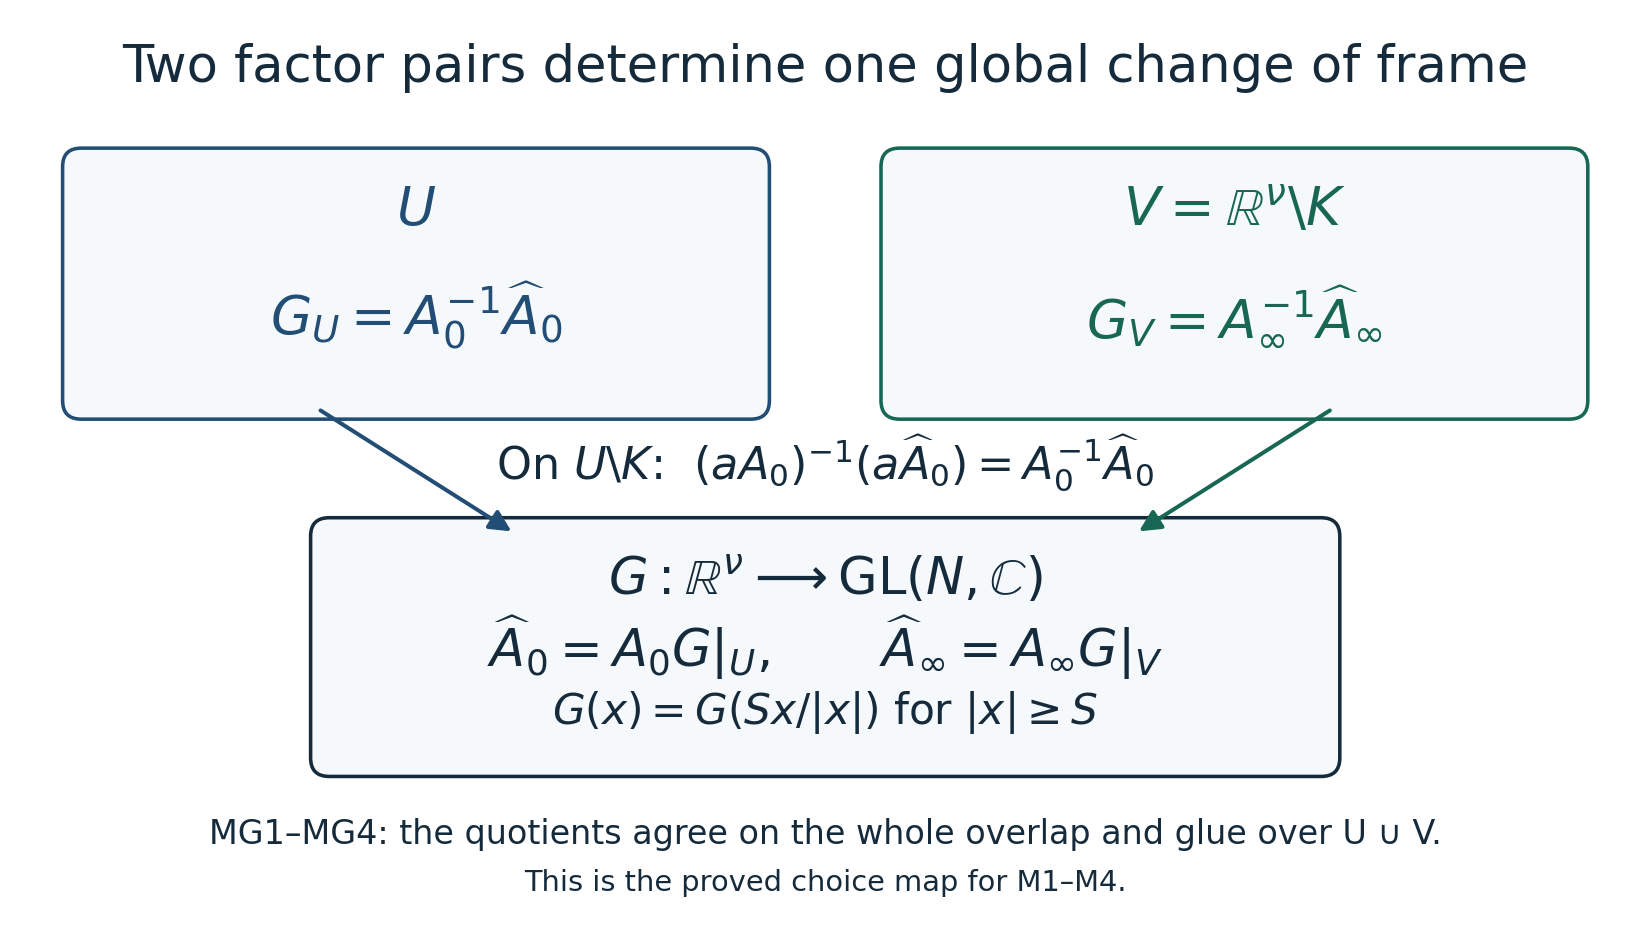
\includegraphics[keepaspectratio,alt={The two original right quotients agree on U minus K and glue to the unique global invertible map G. The exterior identity keeps the full radius S. Complete proof: MG1--MG4.}]{../figures/matrix-extension-choice-map.png}}
\caption{The two original right quotients agree on U minus K and glue to
the unique global invertible map G. The exterior identity keeps the full
radius S. Complete proof: MG1--MG4.}
\end{figure}

The diagram displays the exact map between two factor pairs for the same
original transition. The quotient identities, global domain, inverse and
exterior homogeneity are proved in (MG1)--(MG4). Its reproducible figure
source is matrix-extension-choice-map.py.

Conversely, any smooth invertible \(G\) on \(\mathbb R^\nu\) homogeneous
of degree zero near infinity gives a new valid pair by (MG3). The
domains remain the original \(U,V\), and \(a(A_0G)=(aA_0)G=A_\infty G\).
Outside one radius large enough for both maps their product and its
inverse are homogeneous of degree zero. For two such maps the
consecutive changes are \((A_0G)H=A_0(GH)\) and
\((A_\infty G)H=A_\infty(GH)\), retaining their order. Thus the space of
all valid factor pairs has a free transitive right action by the group
of these global maps: existence of the connecting map is (MG1)--(MG4);
uniqueness follows already from its two restrictions; and if a pair is
unchanged, multiplication by its inverses gives \(G=I_N\) on both cover
members. A free transitive action means that any two pairs are related
by precisely one group element. This is the complete mathematical
content of choice dependence, and (M32) is its constant-map case.

For the jointly smooth families (M34)--(M38), the same calculation gives
a jointly smooth global \(G(x,z)\). If the two families each have a
fixed exterior radius, then one common \(S\) works for all \(z\). On
every compact \(L\Subset Z\), compact-sphere and compact-ball maxima
give all retained \(x\)- and \(z\)-derivative bounds for \(G,G^{-1}\).
There is no bound asserted over a noncompact parameter set. The
parameter base need not itself be contractible: the initial fiber over
\((0,z)\) already has the same chosen chart coordinates for every \(z\).

The relation also preserves the precise compact-support maps needed in
an operator application. Let
\(\mathcal D(U)=C_c^\infty(U;\mathbb C^N)\). Multiplication by \(A_0\)
is a bijection \(\mathcal D(U)\to\mathcal D(U)\), inverse multiplication
by \(A_0^{-1}\), because both are smooth on the original open set. For
any \(u\), invertibility gives \(A_0(x)u(x)=0\) if and only if
\(u(x)=0\), so the support is exactly unchanged. No bound at
\(\partial U\) is needed for this assertion. If
\(P:\mathcal D(U)\to\mathcal D(U)\) is a linear operator, then \[
 \begin{aligned}
 \ker(PA_0)&\longrightarrow\ker P,& u&\longmapsto A_0u,\\
 \ker P&\longrightarrow\ker(PA_0),& v&\longmapsto A_0^{-1}v,\\
 (PA_0)(\mathcal D(U))&=P(\mathcal D(U)),&&\\
 \mathcal D(U)/(PA_0)(\mathcal D(U))
   &\longrightarrow\mathcal D(U)/P(\mathcal D(U)),&[f]&\longmapsto[f]
 \end{aligned}
 \tag{MG5}
\] have the displayed domains, codomains and mutually inverse kernel
maps; the quotient map is the identity on the identical range quotient.
The kernel equality is verified by substitution in each direction, and
the range equality uses the surjectivity of the multiplication map. If
these two dimensions are finite, their actual difference is identical
before and after the right composition. This proves the comparison used
by the later \href{bott-suspension.pdf}{Bott and Euclidean index
reduction}, Remark 13.2, without asserting its separate finiteness or
Fredholm arguments here.

\subsubsection{Smooth families on the original fixed
domains}\label{smooth-families-on-the-original-fixed-domains}

\textbf{Editorial strengthening from the transport proof.} Let
\(Z\subset\mathbb R^d\) be any open parameter set and retain the same
bounded open \(U\), compact \(K\subset U\), and rank \(N\). If \[
 a:(U\setminus K)\times Z\longrightarrow\operatorname{GL}(N,\mathbb C)
 \tag{M34}
\] is smooth jointly in its displayed variables, there are jointly
smooth invertible factors \[
 A_0:U\times Z\longrightarrow\operatorname{GL}(N,\mathbb C),\qquad
 A_\infty:(\mathbb R^\nu\setminus K)\times Z\longrightarrow\operatorname{GL}(N,\mathbb C)
 \tag{M35}
\] with the original ordered identity \[
 A_\infty(x,z)=a(x,z)A_0(x,z)\quad(x\in U\setminus K),\qquad
 A_\infty(x,z)=A_\infty(2Rx/|x|,z)\quad(|x|\geq2R).
 \tag{M36}
\] Here \(R\) is one fixed radius for the whole parameter set, chosen
from the same bounded \(U\). No compactness of \(Z\), extension of \(a\)
across \(K\), or bound near an omitted boundary is assumed.

\textbf{Proof.} Keep exactly the cutoff \(\psi\), open neighborhood
\(W\), and exterior map \(h\) of (M5) and (M26), independent of \(z\).
Glue \(U\times Z\times\mathbb C^N\) and \(V\times Z\times\mathbb C^N\)
by \(v=a(x,z)u\). The two smooth charts and their inverse transitions
verify the bundle structure as in Section 3. In the formulas (M14), take
\(d_xa\), the derivative in the original base coordinates, and retain
the order of its factors. Their zero extensions are jointly smooth: on
\(W\) the first prefactor vanishes identically for every parameter,
while the second has its support in the same compact subset of \(U\).
Formula (M15) and the transport equation (M18) hold with \(d_xa\) along
every path with fixed \(z\).

Choose one of \(U,V\) containing the origin and, in that chart, identify
\(\mathbb C^N\) with the fiber over \((0,z)\) by the identity coordinate
matrix for every \(z\). This is a globally smooth initial frame over
\(Z\). For a fixed endpoint \(x_*\), the finite chart itinerary of
Section 4 depends only on the radial path in the original base; the same
itinerary works for every parameter. On its endpoint neighborhood the
matrices \(-\omega_{O_j}(tx,z)[x]\) are smooth in \((t,x,z)\). On each
compact subset of the endpoint and parameter neighborhoods, their
derivatives have finite bounds. Apply (M7)--(M9) with combined
parameters \((x,z)\): every differentiated transport series converges
uniformly there. Each transition is \(a(t_jx,z)\), its inverse, or the
identity, in the exact order (M24). Thus the transported frame and its
inverse are jointly smooth locally everywhere. The subdivision and
chart-change identities prove agreement of these local descriptions, as
before. Its coordinate matrices satisfy \(F_V(x,z)=a(x,z)F_U(x,z)\).

Set \(A_0(x,z)=F_U(x,z)\) and \(A_\infty(x,z)=F_V(h(x),z)\). The fixed
inclusion \(h(V)\subset V\), the identity \(h|_U=\operatorname{id}\),
and the fixed exterior formula for \(h\) prove every assertion in
(M35)--(M36), including invertibility and the complete factor order.

There is also parameter control of every exterior derivative. Put
\(H(x,z)=F_V(2Rx/|x|,z)\) for \(x\ne0\). For a compact \(L\Subset Z\)
and base and parameter multiindices \(\alpha,\beta\), define the finite
constants \[
 \begin{aligned}
 C_{\alpha,\beta,L}&=(2R)^{|\alpha|}
  \max_{|x|=2R,\ z\in L}\|\partial_x^\alpha\partial_z^\beta H(x,z)\|,\\
 D_{\alpha,\beta,L}&=(2R)^{|\alpha|}
  \max_{|x|=2R,\ z\in L}\|\partial_x^\alpha\partial_z^\beta H(x,z)^{-1}\|.
 \end{aligned}
 \tag{M37}
\] Smoothness on the compact sphere times \(L\) makes these maxima
finite. Differentiate the exact identity \(H(tx,z)=H(x,z)\), first in
\(z\) and then in \(x\). It gives the same power \(t^{-|\alpha|}\) for
both differentiated families, including the inverse. Since
\(H=A_\infty\) on the original exterior, \[
 \begin{aligned}
 \|\partial_x^\alpha\partial_z^\beta A_\infty(x,z)\|
   &\leq C_{\alpha,\beta,L}|x|^{-|\alpha|},\\
 \|\partial_x^\alpha\partial_z^\beta A_\infty(x,z)^{-1}\|
   &\leq D_{\alpha,\beta,L}|x|^{-|\alpha|}
   \quad(|x|\geq2R,\ z\in L).
 \end{aligned}
 \tag{M38}
\] These are the full original exterior derivative estimates, with each
parameter derivative retained. No uniform estimate over noncompact \(Z\)
has been inserted. \(\square\)

\begin{figure}
\centering
\pandocbounded{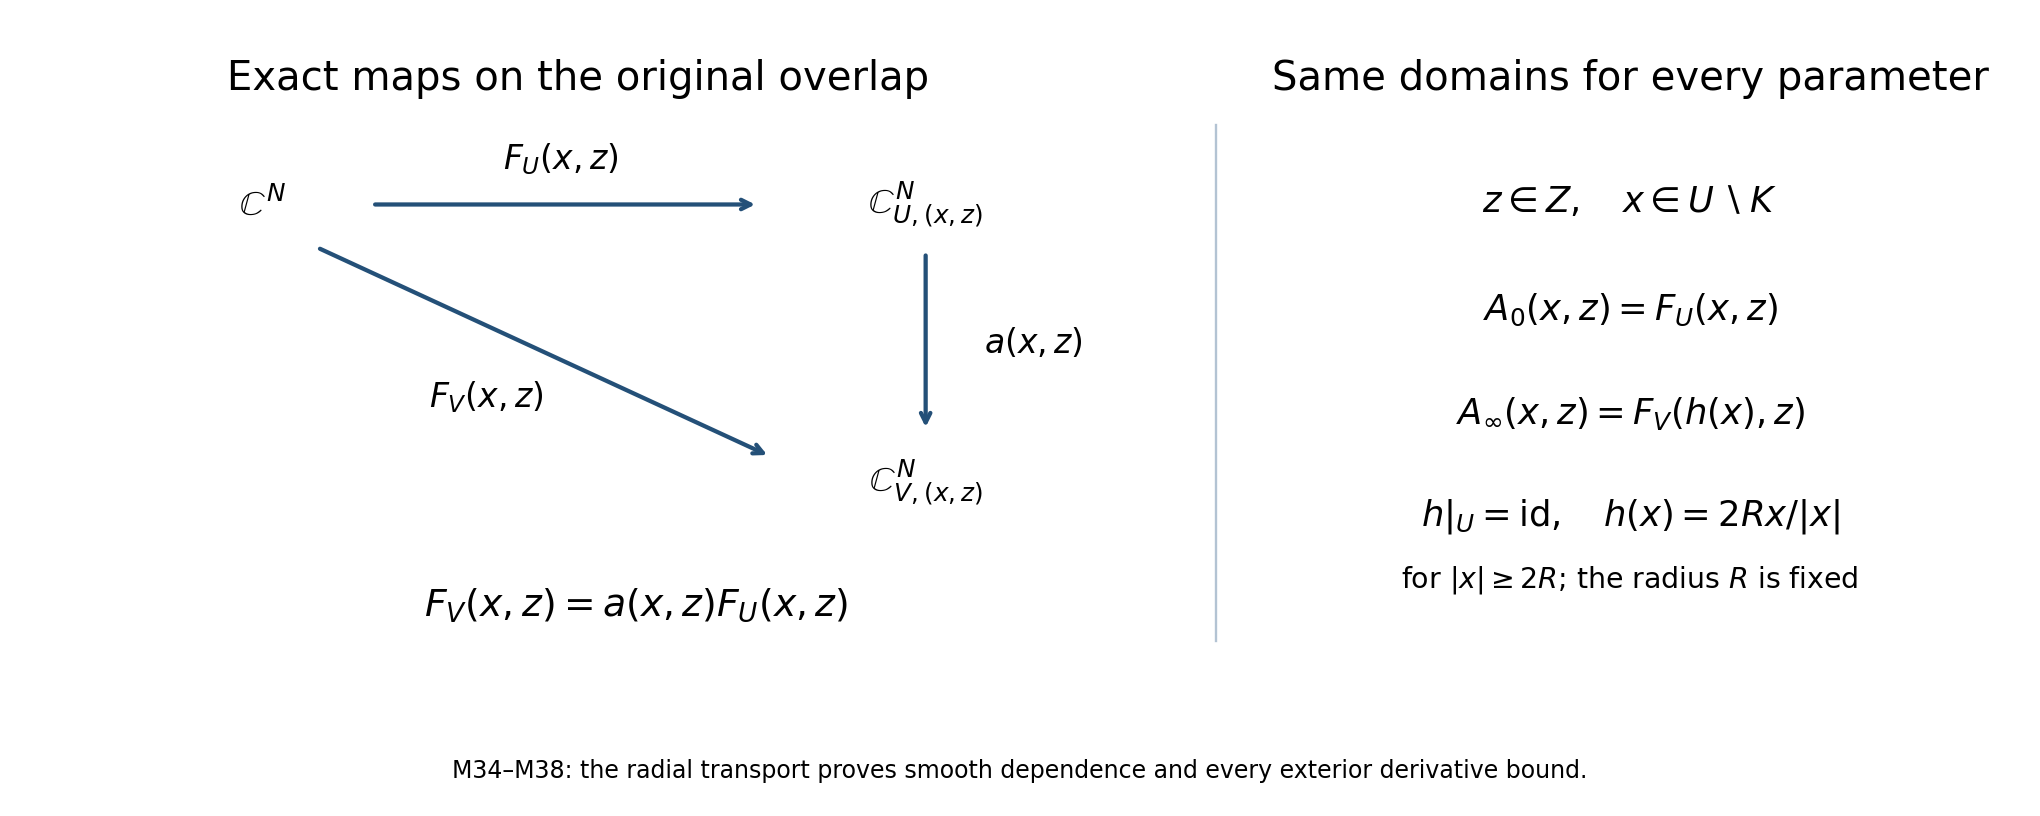
\includegraphics[keepaspectratio,alt={The fixed-domain family keeps its ordered transition while transport supplies a frame at every parameter.}]{../figures/matrix-extension-parameters.png}}
\caption{The fixed-domain family keeps its ordered transition while
transport supplies a frame at every parameter.}
\end{figure}

The two charts lie over the same fixed original domains for every \(z\).
Their frame columns are related by the original \(a(x,z)\), and only the
exterior radius is frozen. The exact family maps, construction and all
derivative bounds are (M34)--(M38).

\subsection{References}\label{references}

The bundle, connection and transport proof above is written out in full
here. The matrix factorization supplies one input to the later
\href{global-elliptic-symbol-index.pdf}{closed-manifold symbol and index
lesson}; it does not by itself establish that lesson's index identity.

Michael Baake and Ulrike Schlägel,
\href{https://arxiv.org/abs/1011.1775v3}{\emph{The Peano--Baker series},
arXiv:1011.1775v3}, revised 20 July 2025; \emph{Proceedings of the
Steklov Institute of Mathematics} 275 (2011), 167--171. Section 2
supplies the ordered-series comparison and the first example of Section
4 supplies (MP1). The full coefficient induction, smooth parameter
endpoint, exponential comparison, inverse-series derivatives and exact
frame-choice maps above are proved here. The cited paper's
original-author TeX was read; its source archive remains private and its
text is not reproduced in this
course.

\end{document}
